% llm-matmeta — formalism and algorithms
% Build: xelatex formalism.tex  (twice, for cross-references; lualatex also works)
\documentclass[11pt,a4paper]{article}

% ---------------------------------------------------------------- fonts
\usepackage{mathpazo}                 % Palatino-style math, matches TeX Gyre Pagella
\usepackage[no-math]{fontspec}
\setmainfont{TeX Gyre Pagella}
\newfontfamily\headfont{Fira Sans}[Ligatures=TeX,UprightFont=*-Regular,BoldFont=*-SemiBold,ItalicFont=*-Italic]
\newfontfamily\headlight{Fira Sans Light}[Ligatures=TeX]
\setmonofont{DejaVu Sans Mono}[Scale=0.82]
\setsansfont{Fira Sans}[Ligatures=TeX,UprightFont=*-Regular,BoldFont=*-SemiBold,ItalicFont=*-Italic]

% ---------------------------------------------------------------- layout
\usepackage[a4paper,margin=2.5cm,top=2.6cm,bottom=2.8cm,headsep=0.8cm]{geometry}
\usepackage{microtype}
\usepackage{amsmath,amssymb,mathtools,amsthm,thmtools}
\usepackage[dvipsnames]{xcolor}
\usepackage{tikz}
\usetikzlibrary{positioning,arrows.meta,calc,fit,backgrounds,shapes.geometric}
\usepackage[most]{tcolorbox}
\usepackage{booktabs,tabularx,array,multirow}
\usepackage{enumitem}
\usepackage[ruled,vlined,linesnumbered]{algorithm2e}
\usepackage{titlesec}
\usepackage{fancyhdr}
\usepackage{listings}
\usepackage{caption}
\usepackage[hidelinks]{hyperref}
\usepackage[nameinlink,capitalise]{cleveref}

% ---------------------------------------------------------------- palette
\definecolor{ink}{HTML}{1F2A37}
\definecolor{accent}{HTML}{1D4E89}
\definecolor{parser}{HTML}{1B7F5B}   % rule-based parser quantities
\definecolor{llm}{HTML}{C2571A}      % LLM quantities
\definecolor{evid}{HTML}{6B46C1}     % evidence / source text
\definecolor{quote}{HTML}{B4237A}    % quotes
\definecolor{merged}{HTML}{1D4E89}   % final record
\definecolor{soft}{HTML}{F3F6FA}
\definecolor{rule}{HTML}{C9D3DF}
\color{ink}

% ---------------------------------------------------------------- notation macros
\newcommand{\rP}{\textcolor{parser}{r_{\mathrm{P}}}}
\newcommand{\rM}{\textcolor{llm}{r_{\mathrm{M}}}}
\newcommand{\rF}{\textcolor{merged}{r}}
\newcommand{\Ev}{\textcolor{evid}{\mathcal{E}}}
\newcommand{\Src}{\textcolor{evid}{T}}
\newcommand{\Qt}{\textcolor{quote}{q}}
\newcommand{\Prov}{\textcolor{merged}{\pi}}
\newcommand{\Conf}{\textcolor{merged}{\mathcal{C}}}
\newcommand{\Model}{\textcolor{llm}{\mathsf{M}}}
\newcommand{\Pars}{\textcolor{parser}{\mathsf{P}}}
\newcommand{\Fset}{\mathbb{F}}
\newcommand{\Vset}{\mathbb{V}}
\newcommand{\nil}{\varnothing}
\newcommand{\valid}{\mathsf{V}}
\newcommand{\agree}{\mathrel{\simeq}}
\newcommand{\norm}{\nu}
\newcommand{\vtag}[1]{\texttt{#1}}
\newcommand{\code}[1]{\texttt{#1}}
\DeclareMathOperator{\Nums}{\mathcal{N}}

% ---------------------------------------------------------------- headings
\titleformat{\section}{\headfont\Large\bfseries\color{accent}}{\thesection}{0.8em}{}
\titleformat{\subsection}{\headfont\large\bfseries\color{ink}}{\thesubsection}{0.7em}{}
\titleformat{\subsubsection}{\headfont\normalsize\bfseries\color{ink}}{\thesubsubsection}{0.6em}{}
\titlespacing*{\section}{0pt}{2.2ex plus .5ex}{1.2ex}
\titlespacing*{\subsection}{0pt}{1.8ex plus .4ex}{0.8ex}

\setlength{\headheight}{22pt}
\pagestyle{fancy}
\fancyhf{}
\renewcommand{\headrulewidth}{0.4pt}
\renewcommand{\headrule}{\hbox to\headwidth{\color{rule}\leaders\hrule height \headrulewidth\hfill}}
\fancyhead[L]{\headfont\small\color{accent}llm-matmeta}
\fancyhead[R]{\headfont\small\color{ink!70}Formalism and algorithms \textbar{} v0.2.0}
\fancyfoot[C]{\headfont\small\color{ink!70}\thepage}

\captionsetup{font={small},labelfont={bf,sf,color=accent},labelsep=period}
\setlist{itemsep=2pt,topsep=4pt}
\SetAlFnt{\small}
\SetAlCapFnt{\small\headfont\bfseries}
\SetAlCapNameFnt{\small\headfont}
\SetKwInOut{Input}{input}\SetKwInOut{Output}{output}

\lstset{basicstyle=\ttfamily\small,columns=fullflexible,keepspaces=true,
  backgroundcolor=\color{soft},frame=single,rulecolor=\color{rule},framesep=4pt,
  xleftmargin=4pt,xrightmargin=4pt,showstringspaces=false}

% ---------------------------------------------------------------- boxes
\tcbset{fbox/.style={enhanced,breakable,boxrule=0.5pt,arc=2pt,left=8pt,right=8pt,top=5pt,bottom=5pt,
  colback=soft,colframe=rule,fonttitle=\headfont\bfseries\small,coltitle=white}}
\newtcbtheorem[number within=section]{defn}{Definition}{fbox,colframe=accent!80,colbacktitle=accent!85}{def}
\newtcbtheorem[use counter from=defn]{prop}{Proposition}{fbox,colframe=parser!80,colbacktitle=parser!85}{prop}
\newtcbtheorem[use counter from=defn]{rem}{Remark}{fbox,colframe=llm!80,colbacktitle=llm!85}{rem}
\newtcolorbox{keybox}{enhanced,boxrule=0pt,arc=0pt,leftrule=3pt,colframe=accent,colback=soft,
  left=10pt,right=8pt,top=6pt,bottom=6pt}

\begin{document}

% ================================================================ title
\thispagestyle{empty}
\begin{tikzpicture}[remember picture,overlay]
  \fill[accent] (current page.north west) rectangle ([yshift=-6.3cm]current page.north east);
  \fill[accent!70!black] ([yshift=-6.3cm]current page.north west) rectangle ([yshift=-6.5cm]current page.north east);
  \node[anchor=north west,text=white,align=left,inner sep=0pt] at ([xshift=2.5cm,yshift=-1.8cm]current page.north west)
  {{\headlight\fontsize{30}{34}\selectfont llm-matmeta}\\[10pt]
   {\headfont\Large Formalism and algorithms}\\[6pt]
   {\headlight\large Hybrid rule-based and LLM metadata extraction for computational materials science}};
\end{tikzpicture}
\vspace*{5.4cm}

\noindent{\headfont\large Gokaran Shukla}\\[2pt]
{\headfont\small\color{ink!75}King Abdullah University of Science and Technology (KAUST), Thuwal, Saudi Arabia}\\[2pt]
{\headfont\small\color{ink!75}Software version 0.2.0 \textbullet{} November 2026 \textbullet{} \url{https://github.com/Gokaran-Shukla/llm-matmeta}}

\vspace{1.0cm}
\begin{keybox}
\noindent{\headfont\bfseries Abstract.}\;
This document gives a precise description of what \code{llm-matmeta} computes. A metadata record is a
partial map from schema field paths to values. A deterministic parser \(\Pars\) and a language model
\(\Model\) each produce such a map from the same files; the model sees only an \emph{evidence} text
\(\Ev\) extracted by the parser, never the parser's own answer. The two maps are merged under a
parser-dominant rule that records the provenance of every field and the set of disagreements.
For files with no parser, the model is the only reader, and every value it returns must be
accompanied by the source line it was read from; a value whose line is not in the file, or does not
contain the value, is flagged or removed. We define each operator, state the guarantees the
construction gives and those it does not, and list the conventions used for VASP, Quantum ESPRESSO,
Wannier90 and batch job scripts.
\end{keybox}

\vspace{0.6cm}
\noindent{\headfont\bfseries\color{accent} Colour convention.}\enspace
Throughout, quantities from the parser are \textcolor{parser}{\bfseries green} (\(\rP\), \(\Pars\)), quantities from the
language model \textcolor{llm}{\bfseries orange} (\(\rM\), \(\Model\)), source and evidence text \textcolor{evid}{\bfseries violet}
(\(\Src\), \(\Ev\)), quotes \textcolor{quote}{\bfseries magenta} (\(\Qt\)), and the final merged record with its
provenance and conflict set \textcolor{merged}{\bfseries blue} (\(\rF\), \(\Prov\), \(\Conf\)).

\vspace{0.6cm}
{\headfont\small
\setlength{\columnsep}{1.2cm}
\noindent\begin{minipage}{\linewidth}
\renewcommand{\contentsname}{\headfont\large\bfseries\color{accent}Contents}
\tableofcontents
\end{minipage}}

\newpage
% ================================================================ 1
\section{Overview}\label{sec:overview}

\Cref{fig:pipeline} shows the two extraction paths. For a calculation directory (VASP) or input file
(Quantum ESPRESSO) the \emph{hybrid path} runs a parser and a model independently and merges them. For any
other text file the \emph{LLM-only path} runs the model alone and checks each value against a quoted line.
Records from the second path can be attached to a calculation record as parts of the same run.

\begin{figure}[h]
\centering
\begin{tikzpicture}[
  font=\headfont\footnotesize, >={Stealth[length=2.2mm]},
  box/.style={rounded corners=2pt, draw=#1!80, fill=#1!9, line width=0.7pt, minimum height=10mm,
    text width=19mm, align=center, inner sep=2pt},
  box/.default=ink,
  data/.style={rounded corners=5pt, draw=#1!75, fill=white, line width=0.6pt, densely dashed,
    minimum height=8mm, text width=20mm, align=center, inner sep=2pt},
  arr/.style={->, line width=0.7pt, draw=#1},
  lab/.style={font=\headfont\scriptsize, text=ink!75, inner sep=1.5pt}]
  % ---------------- hybrid path
  \node[box=evid]   (files) at (0,0)        {raw files\\[-2pt]{\scriptsize INCAR, POSCAR, KPOINTS, OUTCAR}};
  \node[box=parser] (pars)  at (2.6,0)     {parser \(\Pars\)\\[-2pt]{\scriptsize streamed, exact}};
  \node[data=parser](rp)    at (5.2,0.85)   {record \(\rP\)};
  \node[data=evid]  (ev)    at (5.2,-0.85)  {evidence \(\Ev\)};
  \node[box=llm]    (mod)   at (7.8,-0.85) {model \(\Model\)\\[-2pt]{\scriptsize sees schema + \(\Ev\)}};
  \node[box=ink]    (val)   at (10.4,-0.85) {validate \(\valid_S\)\\[-2pt]{\scriptsize one repair round}};
  \node[box=merged] (mer)   at (10.4,0.85)  {merge \(\oplus\)\\[-2pt]{\scriptsize parser dominant}};
  \node[data=merged](out)   at (13.0,0.85) {\(\rF,\ \Prov,\ \Conf\)\\[-2pt]{\scriptsize JSON / JSON-LD}};
  \draw[arr=ink]    (files) -- (pars);
  \draw[arr=parser] (pars.north) |- (rp.west);
  \draw[arr=evid]   (pars.south) |- (ev.west);
  \draw[arr=evid]   (ev) -- (mod);
  \draw[arr=llm]    (mod) -- node[lab, above]{\(\rM\)} (val);
  \draw[arr=parser] (rp) -- (mer);
  \draw[arr=llm]    (val) -- node[lab, left, align=right]{valid \(\rM\)\\or \(\nil\)} (mer);
  \draw[arr=merged] (mer) -- (out);
  % ---------------- LLM-only path
  \node[box=evid]   (tf)    at (0,-3.6)     {any text file \(\Src\)\\[-2pt]{\scriptsize .wout, job script, \dots}};
  \node[box=evid]   (cond)  at (2.6,-3.6)  {condense \(K\)\\[-2pt]{\scriptsize head, tail, keywords}};
  \node[box=llm]    (mod2)  at (5.2,-3.6)   {model \(\Model\)\\[-2pt]{\scriptsize record + quotes}};
  \node[box=quote]  (chk)   at (9.1,-3.6)   {quote check \(\lambda\)\\[-2pt]{\scriptsize against the full \(\Src\)}};
  \node[data=merged](out2)  at (13.0,-3.6) {\(\rF,\ \Prov\)\\[-2pt]{\scriptsize + \code{unverified}}};
  \draw[arr=ink]    (tf) -- (cond);
  \draw[arr=evid]   (cond) -- (mod2);
  \draw[arr=llm]    (mod2) -- node[lab, above]{\((\rM,\Qt)\)} (chk);
  \draw[arr=merged] (chk) -- (out2);
  \draw[->, evid, line width=0.5pt, densely dotted] (tf.south) -- ++(0,-0.45) -| node[lab, pos=0.27, below]{full text, for verification} (chk.south);
  \draw[->, merged, line width=0.6pt, densely dashed] (out2.north) -- node[lab, left, align=right, pos=0.45]{\code{--extras}:\\attachments} (out.south);
  % ---------------- panels
  \begin{scope}[on background layer]
    \node[fit=(files)(rp)(ev)(out)(val), inner xsep=3mm, inner ysep=3mm, rounded corners=4pt, fill=soft] (bg1) {};
    \node[fit=(tf)(out2)(chk), inner xsep=3mm, inner ysep=3mm, yshift=-1.6mm, minimum height=19mm, rounded corners=4pt, fill=soft] (bg2) {};
  \end{scope}
  \node[anchor=south west, font=\headfont\scriptsize\bfseries, text=accent, inner sep=1.5pt] at (bg1.north west) {HYBRID PATH \quad\mdseries\code{matmeta calc}};
  \node[anchor=south west, font=\headfont\scriptsize\bfseries, text=accent, inner sep=1.5pt] at (bg2.north west) {LLM-ONLY PATH \quad\mdseries\code{matmeta file}};
\end{tikzpicture}
\caption{The two extraction paths. On the hybrid path the model never sees \(\rP\), so agreement between \(\rP\) and \(\rM\)
is a genuine second reading. On the LLM-only path there is nothing to compare with; instead each value is
tied to a quoted source line, which is checked against the full file.}
\label{fig:pipeline}
\end{figure}

\paragraph{Design goals.}
(i) \emph{No silent corruption}: an invalid or unreachable model can never change a value the parser found.
(ii) \emph{Traceability}: every field carries a provenance label. (iii) \emph{Bounded context}: the model
sees a few dozen to a few hundred lines, independent of the size of the output file.
(iv) \emph{Locality of data}: any server implementing the OpenAI-style \code{/chat/completions} interface can be used,
including local open-weight models, so files need not leave the institution.

% ================================================================ 2
\section{Records, schemas and validation}\label{sec:records}

\begin{defn}{Field paths and records}{record}
A schema \(S\) defines a finite set of \emph{field paths} \(\Fset_S\), the dotted names of its leaves
(\code{results.total\_energy\_eV}, \code{method.task}, \dots), and for each \(f\in\Fset_S\) a value type
\(\Vset_f\) (number, integer, string, Boolean, array). A \emph{record} is a map
\[
  r:\ \Fset_S \longrightarrow \bigcup_{f}\Vset_f \;\cup\; \{\bot\},\qquad r(f)\in \Vset_f\cup\{\bot\},
\]
where \(\bot\) (JSON \code{null}) means \emph{not stated}. The empty record \(\nil\) has \(\nil(f)=\bot\) for every \(f\).
\end{defn}

The schemas are JSON Schema (draft 2020-12) documents with \code{additionalProperties:false} at every level and
every leaf nullable. Validation is the map
\[
  \valid_S:\ \text{JSON value}\ \longmapsto\ \text{set of error messages},\qquad \valid_S(x)=\varnothing \iff x \text{ conforms to } S.
\]

\paragraph{Conventions are part of the schema.}
Each leaf may carry a \code{description}, and the full schema, descriptions included, is sent to the model.
Descriptions fix conventions that would otherwise produce spurious disagreements, for example:
\begin{itemize}
\item \code{structure.formula} is the formula of the \emph{whole cell}, not reduced, in input order
      (\(\mathrm{Fe_2}\) for a two-atom cell; \(\mathrm{Cu_4In_4P_8S_{24}}\) for four formula units of \(\mathrm{CuInP_2S_6}\)).
\item \code{method.xc\_functional} is the \emph{standard name} of the functional (PBE, PBEsol, SCAN, HSE06, \dots),
      never the raw input tag (VASP \code{GGA = PE} means PBE).
\item \code{method.task} follows VASP's own defaults (\cref{sec:vasp-task}).
\end{itemize}

\begin{table}[h]
\centering\small
\caption{Calculation record (\code{calculation} schema). Units are normalised on extraction.}
\label{tab:calc}
\begin{tabularx}{\linewidth}{@{}l>{\raggedright\arraybackslash}Xl@{}}
\toprule
\headfont Group & \headfont Fields & \headfont Units \\
\midrule
software  & \code{name}, \code{version} & --- \\
method    & \code{task}, \code{xc\_functional}, \code{spin\_polarized}, \code{spin\_orbit\_coupling}, \code{noncollinear},
            \code{hubbard\_u}, \code{van\_der\_waals\_correction} & --- \\
structure & \code{formula}, \code{n\_atoms}, \code{species}, \code{lattice\_vectors\_angstrom} & \AA \\
numerics  & \code{plane\_wave\_cutoff\_eV}, \code{kpoint\_mesh}, \code{smearing\_type}, \code{smearing\_width\_eV},
            \code{energy\_convergence\_eV} & eV \\
results   & \code{converged}, \code{total\_energy\_eV}, \code{energy\_sigma0\_eV}, \code{fermi\_energy\_eV},
            \code{total\_magnetization\_muB}, \code{magnetization\_vector\_muB} & eV, \(\mu_{\mathrm B}\) \\
\bottomrule
\end{tabularx}
\end{table}

% ================================================================ 3
\section{Rule-based parsing}\label{sec:parsing}

The parser is a map \(\Pars: \text{files}\to(\rP,\Ev)\) producing a partial record and an evidence text.
It never calls the model.

\subsection{Streaming output files}
Output files are read in one pass, line by line, through a fixed set of matchers. For every quantity that must
be taken from the \emph{last} occurrence (energies, Fermi level, moments) the parser keeps a bounded queue of the
last \(k\) matching lines (\(k\le 2\)); for parameters it keeps the \emph{first} occurrence. Hence
\[
  \text{time} = O(n),\qquad \text{memory} = O(1)\ \text{in the number of lines } n,
\]
and gzip-compressed files (\code{OUTCAR.gz}) are read transparently. A multi-gigabyte molecular-dynamics
OUTCAR is therefore no harder than a short SCF run.

\subsection{Effective VASP parameters}\label{sec:vasp-tags}
Let \(\tau_{\mathrm{I}}\) be the tags written in the INCAR and \(\tau_{\mathrm{O}}\) the parameters echoed in the
OUTCAR header, which are the values VASP actually used, defaults included. The parser works with the
\emph{effective} tags
\begin{equation}
  \tau \;=\; \tau_{\mathrm{O}} \lhd \tau_{\mathrm{I}},\qquad
  (\tau_{\mathrm{O}}\lhd\tau_{\mathrm{I}})(k)=\begin{cases}\tau_{\mathrm{I}}(k) & k\in\operatorname{dom}\tau_{\mathrm{I}},\\ \tau_{\mathrm{O}}(k) & \text{otherwise,}\end{cases}
  \label{eq:tags}
\end{equation}
so an explicit INCAR value wins, and every tag the INCAR leaves out is taken from what VASP reports.
The harvested OUTCAR parameters are \vtag{IBRION}, \vtag{NSW}, \vtag{ISIF}, \vtag{ISPIN}, \vtag{ICHARG}, \vtag{ISMEAR},
\vtag{SIGMA}, \vtag{ENCUT}, \vtag{EDIFF}, \vtag{LSORBIT}, \vtag{LNONCOLLINEAR}, \vtag{LDAU}, \vtag{IVDW}, \vtag{GGA},
\vtag{LEXCH}, \vtag{METAGGA}, \vtag{LHFCALC}, \vtag{HFSCREEN} and \vtag{LWANNIER90}.

\subsection{Task}\label{sec:vasp-task}
With \(\tau\) from \eqref{eq:tags}, and VASP's own defaults applied when a tag is absent from both sources,
\begin{equation}
 \mathrm{NSW}=\tau(\vtag{NSW})\ \text{or}\ 0,\qquad
 \mathrm{IBRION}=\tau(\vtag{IBRION})\ \text{or}\ \begin{cases}-1 & \mathrm{NSW}\in\{0,-1\}\\ \phantom{-}0 & \text{otherwise}\end{cases}
\end{equation}
and the task is
\begin{equation}
 \mathrm{task}(\tau)=\begin{cases}
 \texttt{nscf} & \vtag{ICHARG}=11,\\
 \texttt{scf} & \mathrm{IBRION}=-1,\ \text{or}\ \mathrm{NSW}=0 \text{ with } \mathrm{IBRION}\in\{0,1,2,3\},\\
 \texttt{vc-relax} & \mathrm{IBRION}\in\{1,2,3\},\ \mathrm{NSW}>0,\ \vtag{ISIF}\in\{3,6,7\},\\
 \texttt{relax} & \mathrm{IBRION}\in\{1,2,3\},\ \mathrm{NSW}>0,\ \text{otherwise},\\
 \texttt{md} & \mathrm{IBRION}=0,\ \mathrm{NSW}>0,\\
 \texttt{phonon} & \mathrm{IBRION}\in\{5,6,7,8\},\\
 \texttt{other} & \text{otherwise}.
 \end{cases}
\end{equation}
Version 0.1 assigned a task only when \vtag{IBRION} was written explicitly, so a static Wannier90 run whose
INCAR omitted it received no task from the parser, and a model filled the gap with \texttt{relax}.

\subsection{Exchange--correlation functional}
\begin{equation}
 \mathrm{xc}(\tau)=\begin{cases}
  \tau(\vtag{METAGGA}) & \vtag{METAGGA}\notin\{\texttt{--},\texttt{NONE},\texttt{F}\},\\
  \text{HSE06} & \vtag{LHFCALC}=\texttt{T},\ |\tau(\vtag{HFSCREEN})-0.2|<10^{-6},\\
  \text{hybrid} & \vtag{LHFCALC}=\texttt{T}\ \text{otherwise},\\
  g\bigl(\tau(\vtag{GGA})\bigr) & \vtag{GGA} \text{ set and } \neq\texttt{--},\\
  g\bigl(\tau(\vtag{LEXCH})\bigr) & \text{otherwise},
 \end{cases}
\end{equation}
where \(g\) translates VASP's codes into standard names:
\(g:\ \texttt{PE}\mapsto\text{PBE},\ \texttt{PS}\mapsto\text{PBEsol},\ \texttt{RP}\mapsto\text{rPBE},\ \texttt{91}\mapsto\text{PW91},\ \texttt{AM}\mapsto\text{AM05},\ \texttt{CA}\mapsto\text{LDA}\).
The \vtag{LEXCH} branch matters in practice: most INCARs set no \vtag{GGA}, and the functional is then
defined by the POTCAR, which VASP reports as \code{LEXCH = PE}.

\subsection{Electronic structure results}
Let \(F\) be the last \emph{free energy} \(\mathrm{TOTEN}\), \(E_0\) the matching \emph{energy without entropy},
and \(E_{\sigma\to0}\) the value VASP prints as \code{energy(sigma->0)}; for its smearing schemes VASP reports
\begin{equation}
  E_{\sigma\to 0} = \tfrac12\,(F + E_0),
\end{equation}
which removes the leading-order smearing error. The record keeps both:
\code{total\_energy\_eV} \(=F\) and \code{energy\_sigma0\_eV} \(=E_{\sigma\to0}\). For metals with large
\(\sigma\), energy differences should be formed from \(E_{\sigma\to0}\).

For the magnetisation, the last line \code{number of electron \(N\) magnetization \(\dots\)} carries one value
(collinear) or three (noncollinear). With \(\mathbf m=(m_x,m_y,m_z)\),
\begin{equation}
 M_{\mathrm{tot}}=\begin{cases} m & \text{collinear},\\ \lVert\mathbf m\rVert=\sqrt{m_x^2+m_y^2+m_z^2} & \text{noncollinear},\end{cases}
\end{equation}
stored as \code{total\_magnetization\_muB}, with \(\mathbf m\) itself stored as \code{magnetization\_vector\_muB}
(noncollinear runs only).
Version 0.1 read only \(m_x\) in noncollinear runs, which reports zero for a moment along \(z\).

\subsection{Structure}
For runs that move atoms (\(\mathrm{task}\in\{\texttt{relax},\texttt{vc-relax},\texttt{md}\}\)) the structure is
read from CONTCAR, the final geometry; otherwise from POSCAR. The file used is recorded in
\code{source.structure\_from}. Lattice vectors are \(\mathbf a_i = s\,\tilde{\mathbf a}_i\) with \(s\) the POSCAR
scale factor, in \AA.

\subsection{Quantum ESPRESSO}
Inputs are read from the namelists and cards; outputs are streamed as above. Energies in Rydberg are converted
with \(1\,\mathrm{Ry}=13.605\,693\,122\,994\,\mathrm{eV}\) (CODATA 2018), so
\(E_{\mathrm{cut}}^{\mathrm{eV}} = E_{\mathrm{cut}}^{\mathrm{Ry}}\cdot\mathrm{Ry}\), and likewise for
\code{conv\_thr} and \code{degauss}. The functional is taken from \code{input\_dft}, or else from the line
\code{Exchange-correlation= \dots} of the output. Noncollinear moments are treated as in VASP.

\subsection{The evidence text}\label{sec:evidence}
The evidence \(\Ev\) is the only text the model sees. It is the concatenation of
\begin{enumerate}[label=(\alph*)]
\item the INCAR \emph{verbatim};
\item the first six lines of the KPOINTS file (a full explicit k-point list is not useful);
\item the header of the structure file (title, scale, lattice, species, counts) \emph{verbatim};
\item from the OUTCAR: the version line, up to six POTCAR lines, the effective-parameter lines of
      \cref{sec:vasp-tags}, the last two \(\mathrm{TOTEN}\) lines, the last \(E_{\sigma\to0}\) line, the last
      \(E_{\mathrm F}\) line, the last two magnetisation lines and the convergence message;
\end{enumerate}
and, for Quantum ESPRESSO, the full \code{pw.x} input plus the corresponding output lines.

\begin{rem}{What is, and is not, an independent second reading}{indep}
Partition the fields as \(\Fset=\Fset_{\mathrm{in}}\sqcup\Fset_{\mathrm{out}}\). Fields in \(\Fset_{\mathrm{in}}\) (settings:
cutoff, smearing, spin, SOC, functional, k-mesh, structure) are derived by the model from \emph{verbatim} input text,
so agreement \(\rM(f)\agree\rP(f)\) is evidence that the parser's interpretation is right. Fields in \(\Fset_{\mathrm{out}}\)
(energies, \(E_{\mathrm F}\), moments, convergence) come from lines the parser itself selected. Agreement there
confirms that the number was read from the selected line correctly, but cannot reveal that the parser selected
the wrong line. Passing the effective-parameter block (d) to the model moves the defaulted tags from the second
category to the first.
\end{rem}

% ================================================================ 4
\section{Querying the model}\label{sec:llm}

The model is used as a function \(\Model(\sigma, u)\mapsto\) JSON object, where \(\sigma\) is a fixed system
prompt and \(u\) the user message (schema, optional instructions, source text, and on a retry the list of
validation errors). Requests use temperature \(0\) and ask the server for a JSON object; replies wrapped in
Markdown code fences or preceded by text are tolerated.

\begin{algorithm}[h]
\caption{\textsc{AskWithRetry}: schema-constrained query with one repair round}\label{alg:ask}
\Input{model \(\Model\), system prompt \(\sigma\), schema \(S\), text \(x\), retries \(R=1\)}
\Output{reply \(y\) and its validation errors \(e\)}
\(y \leftarrow \Model\bigl(\sigma,\ \mathrm{prompt}(S,x)\bigr)\);\quad \(e\leftarrow\valid_S(y)\)\;
\For{\(i=1,\dots,R\)}{
  \lIf{\(e=\varnothing\)}{\textbf{break}}
  \(y \leftarrow \Model\bigl(\sigma,\ \mathrm{prompt}(S,x,e)\bigr)\);\quad \(e\leftarrow\valid_S(y)\)\;
}
\Return{\((y,e)\)}\;
\end{algorithm}

On the hybrid path the model's record is
\begin{equation}
  \rM=\begin{cases} y & \text{if the call succeeded and } e=\varnothing,\\ \nil & \text{if } e\neq\varnothing \text{ or the call raised (network, server, authentication, parse error).}\end{cases}
  \label{eq:rm}
\end{equation}
The error, if any, is reported in \code{llm\_error} and \code{source.llm\_used} is set to \code{false}. With
\(\rM=\nil\) the merge of \cref{sec:merge} returns \(\rP\) unchanged, so a batch run over many directories always
produces a record for every directory, even if the model is down.

% ================================================================ 5
\section{Merge, provenance and conflicts}\label{sec:merge}

\begin{defn}{Agreement}{agree}
For two non-null values of the same field, \(a\agree b\) holds when
\begin{itemize}
\item numbers: \(|a-b|\le\max\!\bigl(\rho\max(|a|,|b|),\ \alpha\bigr)\) with \(\rho=10^{-3}\), \(\alpha=10^{-6}\);
\item strings: equal after trimming and case folding;
\item Booleans: identical (a Boolean never agrees with a number);
\item arrays: equal length and element-wise \(\agree\) (so lattice vectors are compared with tolerance).
\end{itemize}
\end{defn}

\begin{defn}{Merge}{merge}
The merged record \(\rF\), its provenance \(\Prov:\Fset\to\mathcal L\) and its conflict set \(\Conf\subseteq\Fset\) are
defined field by field:
\begin{center}\small
\begin{tabular}{@{}lll@{}}
\toprule
\headfont condition on \((\rP(f),\,\rM(f))\) & \headfont \(\rF(f)\) & \headfont \(\Prov(f)\) \\
\midrule
both \(\neq\bot\),\ \(\rP(f)\agree\rM(f)\)        & \(\rP(f)\) & \texttt{parser+llm} \\
both \(\neq\bot\),\ \(\rP(f)\not\agree\rM(f)\)    & \(\rP(f)\) & \texttt{parser (llm disagreed)} \\
\(\rP(f)\neq\bot,\ \rM(f)=\bot\)                  & \(\rP(f)\) & \texttt{parser} \\
\(\rP(f)=\bot,\ \rM(f)\neq\bot\)                  & \(\rM(f)\) & \texttt{llm} \\
both \(=\bot\)                                    & \(\bot\)   & \texttt{missing} \\
\bottomrule
\end{tabular}
\end{center}
\[
\Conf=\{\,f\in\Fset:\ \Prov(f)=\texttt{parser (llm disagreed)}\,\},
\]
reported as triples \(\bigl(f,\rP(f),\rM(f)\bigr)\), sorted by \(f\).
\end{defn}

\begin{prop}{Properties of the merge}{props}
\begin{enumerate}[label=(\roman*)]
\item \emph{Parser dominance.} \(\rP(f)\neq\bot\Rightarrow\rF(f)=\rP(f)\). The model can add values, never change them.
\item \emph{Safe failure.} If \(\rM=\nil\) then \(\rF=\rP\) and \(\Conf=\varnothing\).
\item \emph{Validity.} If \(\valid_S(\rP)=\varnothing\) and \(\valid_S(\rM)=\varnothing\), then \(\valid_S(\rF)=\varnothing\).
\item \emph{Order independence.} \(\rF\), \(\Prov\) and \(\Conf\) do not depend on the order in which fields are visited.
\end{enumerate}
\end{prop}
\noindent\emph{Proof sketch.} (i) and (ii) are immediate from the definition and \eqref{eq:rm}. For (iii), the schemas
impose only per-field type constraints (no cross-field constraints), and every \(\rF(f)\) is taken from a record that
satisfies the constraint for \(f\). (iv) holds because each field is decided from \(\rP(f)\) and \(\rM(f)\) alone. \qed

\paragraph{Reading the provenance.} \texttt{parser+llm} is the strongest label: two independent readings agree
(with the caveat of Remark~\ref{rem:indep}). \texttt{llm} marks the only values that rest on the model alone; these are
the ones to inspect. A non-empty \(\Conf\) is the useful output of the cross-check: a misread by the model, a
notational mismatch, or a blind spot of the parser.

% ================================================================ 6
\section{LLM-only extraction with quote verification}\label{sec:quotes}

Without a parser there is no \(\rP\) to compare with. The model is therefore asked to return, together with the
record, the source line each value was read from:
\[
 \Model(\sigma_{\mathrm q}, u)\ \longmapsto\ (\rM,\Qt),\qquad \Qt:\ \Fset\rightharpoonup\text{strings},
\]
validated against the wrapper schema \(\{\texttt{record}: S,\ \texttt{quotes}: \text{map of strings}\}\) with
\cref{alg:ask}. Each value is then checked against the \emph{full} source \(\Src\), not against the excerpt sent to the model.

\subsection{The verification predicate}
Let \(\norm(s)\) collapse all runs of white space in \(s\) to a single space and trim the ends. A quote may span
several lines \(\ell_1,\dots,\ell_m\); write \(\bar q=\norm(\ell_1)\,\cdots\,\norm(\ell_m)\).

\begin{defn}{Quote checks}{qcheck}
For a field \(f\) with value \(v=\rM(f)\) and quote \(\Qt_f\), the quote is \emph{found} when
\[
 \mathsf{found}(\Qt_f) \iff \forall j:\ \norm(\ell_j)\ \text{is a substring of}\ \norm(\Src),
\]
and the value is \emph{contained} in it, \(\mathsf{contains}(v,\bar q)\), when
\begin{itemize}
\item \(v\) is a number and there are \(n\in\Nums(\bar q)\), \(c\in\mathcal U\) with
      \(|c\,n-v|\le\max\!\bigl(10^{-4}\max(|cn|,|v|),\,10^{-8}\bigr)\);
\item \(v\) is a string and \(\norm(v)\), or one of its aliases, is a substring of \(\bar q\) (case-folded);
\item \(v\) is an array and \(\mathsf{contains}(v_i,\bar q)\) holds for every element.
\end{itemize}
Here \(\Nums(\bar q)\) is the set of numbers written in \(\bar q\) (Fortran \code{D} exponents included) and
\(\mathcal U=\{1,\ \mathrm{Ry},\ \mathrm{Ha},\ a_0,\ a_0^2,\ \mathrm{Ry}^{-1}\}\) the accepted unit factors
(\(\mathrm{Ha}=2\,\mathrm{Ry}\), \(a_0=0.529\,177\,210\,903\)\,\AA). Aliases cover values that are named rather
than written, e.g.\ \texttt{slurm} is accepted when the quote contains \code{\#SBATCH} or \code{srun}.
\end{defn}

The provenance label is
\begin{equation}
\lambda(f)=\begin{cases}
\texttt{missing} & v=\bot,\\
\texttt{llm (unverified: no quote)} & v\neq\bot,\ \Qt_f \text{ absent or empty},\\
\texttt{llm (unverified: quote not in file)} & \neg\,\mathsf{found}(\Qt_f),\\
\texttt{llm (quote found)} & \mathsf{found}(\Qt_f),\ v \text{ Boolean},\\
\texttt{llm (verified)} & \mathsf{found}(\Qt_f)\wedge\mathsf{contains}(v,\bar q),\\
\texttt{llm (unverified: value not in quote)} & \text{otherwise.}
\end{cases}
\label{eq:lambda}
\end{equation}
In \emph{strict} mode every unverified value is removed, \(\rF(f)=\bot\), and its label becomes
\texttt{dropped (unverified: \dots)}; otherwise the value is kept and the field is listed in \code{unverified}.

\begin{rem}{What the quote check can and cannot catch}{qlimits}
\emph{Caught:} an invented number with no quote; an invented quote (a plausible line that is not in the file); a
real line paired with a number that is not on it. These are the common failure modes of small models.
\emph{Not caught:} a misattribution, where a number really appears on the quoted line but belongs to another
quantity (for example \(\Omega_{\mathrm D}\) reported as \(\Omega_{\mathrm{tot}}\) when both share a line), or a quote
taken from the wrong part of a file that repeats a pattern (an early iteration instead of the final state).
Booleans can only be checked for the existence of the quoted line. The check is thus a strong filter for
fabrication, not a proof of correctness.
\end{rem}

\subsection{Condensation}\label{sec:condense}
Long files are reduced before they are sent. Let \(\Src\) have lines \(0,\dots,n-1\), let \(W\) be a list of
lower-case keywords for the schema, and let \(H\) be the first \(h_{\max}\) line indices whose text contains a keyword.
With head \(h\), tail \(t\) and context \(c\),
\begin{equation}
  K(\Src)=\begin{cases}\Src & |\Src|\le L,\\[2pt]
  \Src\big|_{I},\quad I=[0,h)\ \cup\ [n-t,n)\ \cup\ \bigcup_{i\in H}[i-c,\,i+c] & \text{otherwise},\end{cases}
\end{equation}
with every gap in \(I\) replaced by a marker \code{[... \(k\) lines skipped ...]}. Defaults are
\(L=24\,000\) characters, \(h=80\), \(t=150\), \(c=1\), \(h_{\max}=300\). The head captures settings that codes print
first, the tail captures final results, and the keyword windows capture everything in between. Because \(\lambda\)
is evaluated against the full \(\Src\), condensation can make a value \texttt{missing} but never makes a fabricated value
pass.

% ================================================================ 7
\section{Record types for files without a parser}\label{sec:schemas}

\begin{table}[h]
\centering\small
\caption{Wannier90 record (\code{wannier} schema), read from \code{seedname.wout}.}
\label{tab:wannier}
\begin{tabularx}{\linewidth}{@{}l>{\raggedright\arraybackslash}X@{}}
\toprule
\headfont Group & \headfont Fields \\
\midrule
software        & \code{name}, \code{version} (release) \\
system          & \code{num\_wann}, \code{num\_bands}, \code{kpoint\_mesh} (MP grid), \code{spinors} \\
disentanglement & \code{used}; outer window \code{outer\_window\_\{min,max\}\_eV}; frozen window \code{frozen\_window\_\{min,max\}\_eV};
                  \code{converged}; \code{final\_omega\_i\_A2} \\
wannierisation  & \code{num\_iter}, \code{converged}, \(\Omega_{\mathrm I}\), \(\Omega_{\mathrm D}\), \(\Omega_{\mathrm{OD}}\),
                  \(\Omega=\Omega_{\mathrm I}+\Omega_{\mathrm D}+\Omega_{\mathrm{OD}}\) (all in \AA\(^2\)) \\
\bottomrule
\end{tabularx}
\end{table}

For the spreads, a record should satisfy the Marzari--Vanderbilt decomposition
\(\Omega=\Omega_{\mathrm I}+\Omega_{\mathrm D}+\Omega_{\mathrm{OD}}\); in the bundled example
\(31.250\,048 + 0.004\,512 + 1.847\,573 = 33.102\,133\,\)\AA\(^2\). This identity is a natural consistency test to add to the
quote check (\cref{sec:roadmap}), because it would catch exactly the misattributions described in Remark~\ref{rem:qlimits}.

\begin{table}[h]
\centering\small
\caption{Batch-job record (\code{jobscript} schema), read from SLURM, PBS, LSF or SGE scripts.}
\label{tab:job}
\begin{tabularx}{\linewidth}{@{}l>{\raggedright\arraybackslash}X@{}}
\toprule
\headfont Group & \headfont Fields \\
\midrule
---       & \code{scheduler}, \code{job\_name} \\
resources & \code{partition}, \code{nodes}, \code{ntasks}, \code{ntasks\_per\_node}, \code{cpus\_per\_task}, \code{gpus},
            \code{memory}, \code{time\_limit}, \code{constraint} \\
software  & \code{modules} (every module loaded, as written), \code{executable} (e.g.\ \code{vasp\_ncl}), \code{launcher} \\
\bottomrule
\end{tabularx}
\end{table}

The job script is valuable beyond bookkeeping: the executable is independent evidence about the calculation
(\code{vasp\_ncl} implies a noncollinear build; the loaded \code{vasp/\(x.y.z\)} module dates the code version).

\paragraph{Detection.} A file is read as \code{wannier} if its suffix is \code{.wout}; as \code{jobscript} if it is
a text file under 200\,kB whose first 20\,kB contain a line starting with \code{\#SBATCH}, \code{\#PBS}, \code{\#BSUB} or
\code{\#\$}, or a shebang together with \code{srun}, \code{mpirun} or \code{mpiexec}; otherwise as a generic
\code{calculation}.

% ================================================================ 8
\section{Composite records and JSON-LD}\label{sec:composite}

With \code{--extras}, a run directory \(D\) yields one composite record
\[
  R(D)=\Bigl(\rF_{\mathrm{calc}},\ \Prov_{\mathrm{calc}},\ \Conf_{\mathrm{calc}},\ \bigl\{(\phi,\kappa_\phi,\rF_\phi,\Prov_\phi)\bigr\}_{\phi\in X(D)}\Bigr),
\]
where \(X(D)\) is the set of detected extra files and \(\kappa_\phi\in\{\texttt{wannier},\texttt{jobscript}\}\) their
record types. A Wannierised SOC calculation is then described once, from the functional and moment to the
spread of the Wannier functions and the executable that produced them.

For export, every field name \(f\) is mapped to an ontology term \(\mathrm{term}(f)\) through a JSON-LD
\code{@context}; null fields are dropped; a field with a unit becomes \(\{\texttt{value}: v,\ \texttt{unit}: u\}\);
and the attachments become \code{hasPart} nodes typed \code{Wannier90Run} or \code{BatchJob}. The default
context uses a placeholder namespace; publishing into a specific knowledge graph means supplying a context that maps
the same field names onto that graph's ontology.

% ================================================================ 9
\section{Worked example: bcc Fe with spin--orbit coupling}\label{sec:example}

The directory \code{examples/vasp\_Fe\_soc} contains an INCAR that sets neither \vtag{IBRION}, \vtag{NSW} nor
\vtag{GGA}, an OUTCAR with a moment along \(z\), a Wannier90 output and a SLURM script. The parser alone gives:

\begin{table}[h]
\centering\small
\caption{Selected parser values for \code{examples/vasp\_Fe\_soc} and the rule that produced them.}
\begin{tabularx}{\linewidth}{@{}llX@{}}
\toprule
\headfont Field & \headfont Value & \headfont Rule \\
\midrule
\code{method.task} & \texttt{scf} & \vtag{IBRION} \(=-1\) from \(\tau_{\mathrm O}\), \cref{sec:vasp-task} \\
\code{method.xc\_functional} & PBE & no \vtag{GGA}; \vtag{LEXCH} \(=\) \texttt{PE} \\
\code{method.noncollinear} & \texttt{true} & implied by \vtag{LSORBIT} \(=\) \texttt{T} \\
\code{numerics.smearing\_type} & Gaussian & \vtag{ISMEAR} \(=0\) \\
\code{results.total\_energy\_eV} & \(-8.295\,312\,07\) & last \(F\) \\
\code{results.energy\_sigma0\_eV} & \(-8.295\,141\,61\) & \(\tfrac12(F+E_0)\), as printed \\
\code{results.magnetization\_vector\_muB} & \((1.1\!\times\!10^{-6},\,-3.1\!\times\!10^{-6},\,2.231)\) & three components \\
\code{results.total\_magnetization\_muB} & \(2.231\,087\) & \(\lVert\mathbf m\rVert\) \\
\bottomrule
\end{tabularx}
\end{table}

\noindent Version 0.1 would have returned no task, no functional, and a total moment of \(1.1\times10^{-6}\,\mu_{\mathrm B}\).

% ================================================================ 10
\section{Command-line interface}

\begin{lstlisting}
matmeta calc     RUN_DIR [...]  [--no-llm] [--extras] [--strict]
                                [--jsonld] [--context CTX.json] [-o DIR]
matmeta file     FILE [...]     [--schema auto|wannier|jobscript|calculation]
                                [--strict] [-o DIR]
matmeta abstract ABSTRACT.txt [...]  [-o DIR]
\end{lstlisting}
The model endpoint is configured with three environment variables, or with the \code{--base-url} and
\code{--model} options:
\begin{center}\small
\begin{tabular}{@{}ll@{}}
\code{MATMETA\_BASE\_URL} & server address, e.g.\ \code{http://localhost:11434/v1} for a local Ollama server \\
\code{MATMETA\_MODEL}     & model name, e.g.\ \code{llama3.1} or \code{qwen2.5:7b} \\
\code{MATMETA\_API\_KEY}  & key for hosted services; not needed for local servers \\
\end{tabular}
\end{center}
Diagnostics go to standard error, one line each: \code{[conflict]} for \(f\in\Conf\), \code{[unverified]} for a
failed quote check, \code{[warning]} for a failed or invalid model reply, and \code{[error]} for an unreadable input.
The JSON written to standard output is unaffected.

% ================================================================ 11
\section{Evaluation metrics and roadmap}\label{sec:roadmap}

For a curated set of runs with gold records \(r^\ast\), the natural per-field scores are
\begin{equation}
 \mathrm{precision}_f=\frac{\#\{\rF(f)\neq\bot,\ \rF(f)\agree r^\ast(f)\}}{\#\{\rF(f)\neq\bot\}},\qquad
 \mathrm{recall}_f=\frac{\#\{\rF(f)\neq\bot,\ \rF(f)\agree r^\ast(f)\}}{\#\{r^\ast(f)\neq\bot\}},
\end{equation}
computed separately for each provenance class, together with the conflict rate \(|\Conf|/|\Fset|\) and, on the
LLM-only path, the verification rate and the precision of \emph{verified} values. Comparing these across models
(local 7--8\,B models, larger hosted models) and across the two paths gives a quantitative answer to how much each
component contributes.

Planned extensions:
\begin{itemize}
\item \emph{Consistency constraints} that are checkable from the record alone, such as
      the spread decomposition \(\Omega=\Omega_{\mathrm I}+\Omega_{\mathrm D}+\Omega_{\mathrm{OD}}\), the atom count
      \(n_{\mathrm{atoms}}=\sum_s n_s\), or the task count \(N_{\mathrm{tasks}}=N_{\mathrm{nodes}}\,N_{\mathrm{tasks/node}}\),
      to catch misattributions.
\item Further rule-based parsers (SIESTA, Wannier90, phonopy, LAMMPS), which move a code from the LLM-only to the hybrid path.
\item Mapping to community ontologies and export to research-data repositories.
\item Extraction from full-text papers, linking each publication to the records of the calculations behind it.
\end{itemize}

\vspace{6mm}
\begin{keybox}\small
\noindent{\headfont\bfseries How to cite.} G.~Shukla, \emph{llm-matmeta: hybrid rule-based and LLM metadata extraction for
computational materials science}, Zenodo, \url{https://doi.org/10.5281/zenodo.24334736}.
\end{keybox}

\end{document}
